We would like to start our thesis with a general description of the communication system, possible vulnerabilities, and the actors participating in it.
Since the task of this thesis is to implement software components that meet the specified security requirements,
namely: web client, web server, mobile client, desktop client and database, then it is these components that will be our
actors.
Communication between the components takes place over the HTTPS protocol.
REST API is used as a backend, and therefore, the format of the data transmitted from the client to the server is JSON\@.
The following diagram describes the basic concept of the system, and conveys the relationships between the actors mentioned above.

\begin{figure}[H]
    \centering
    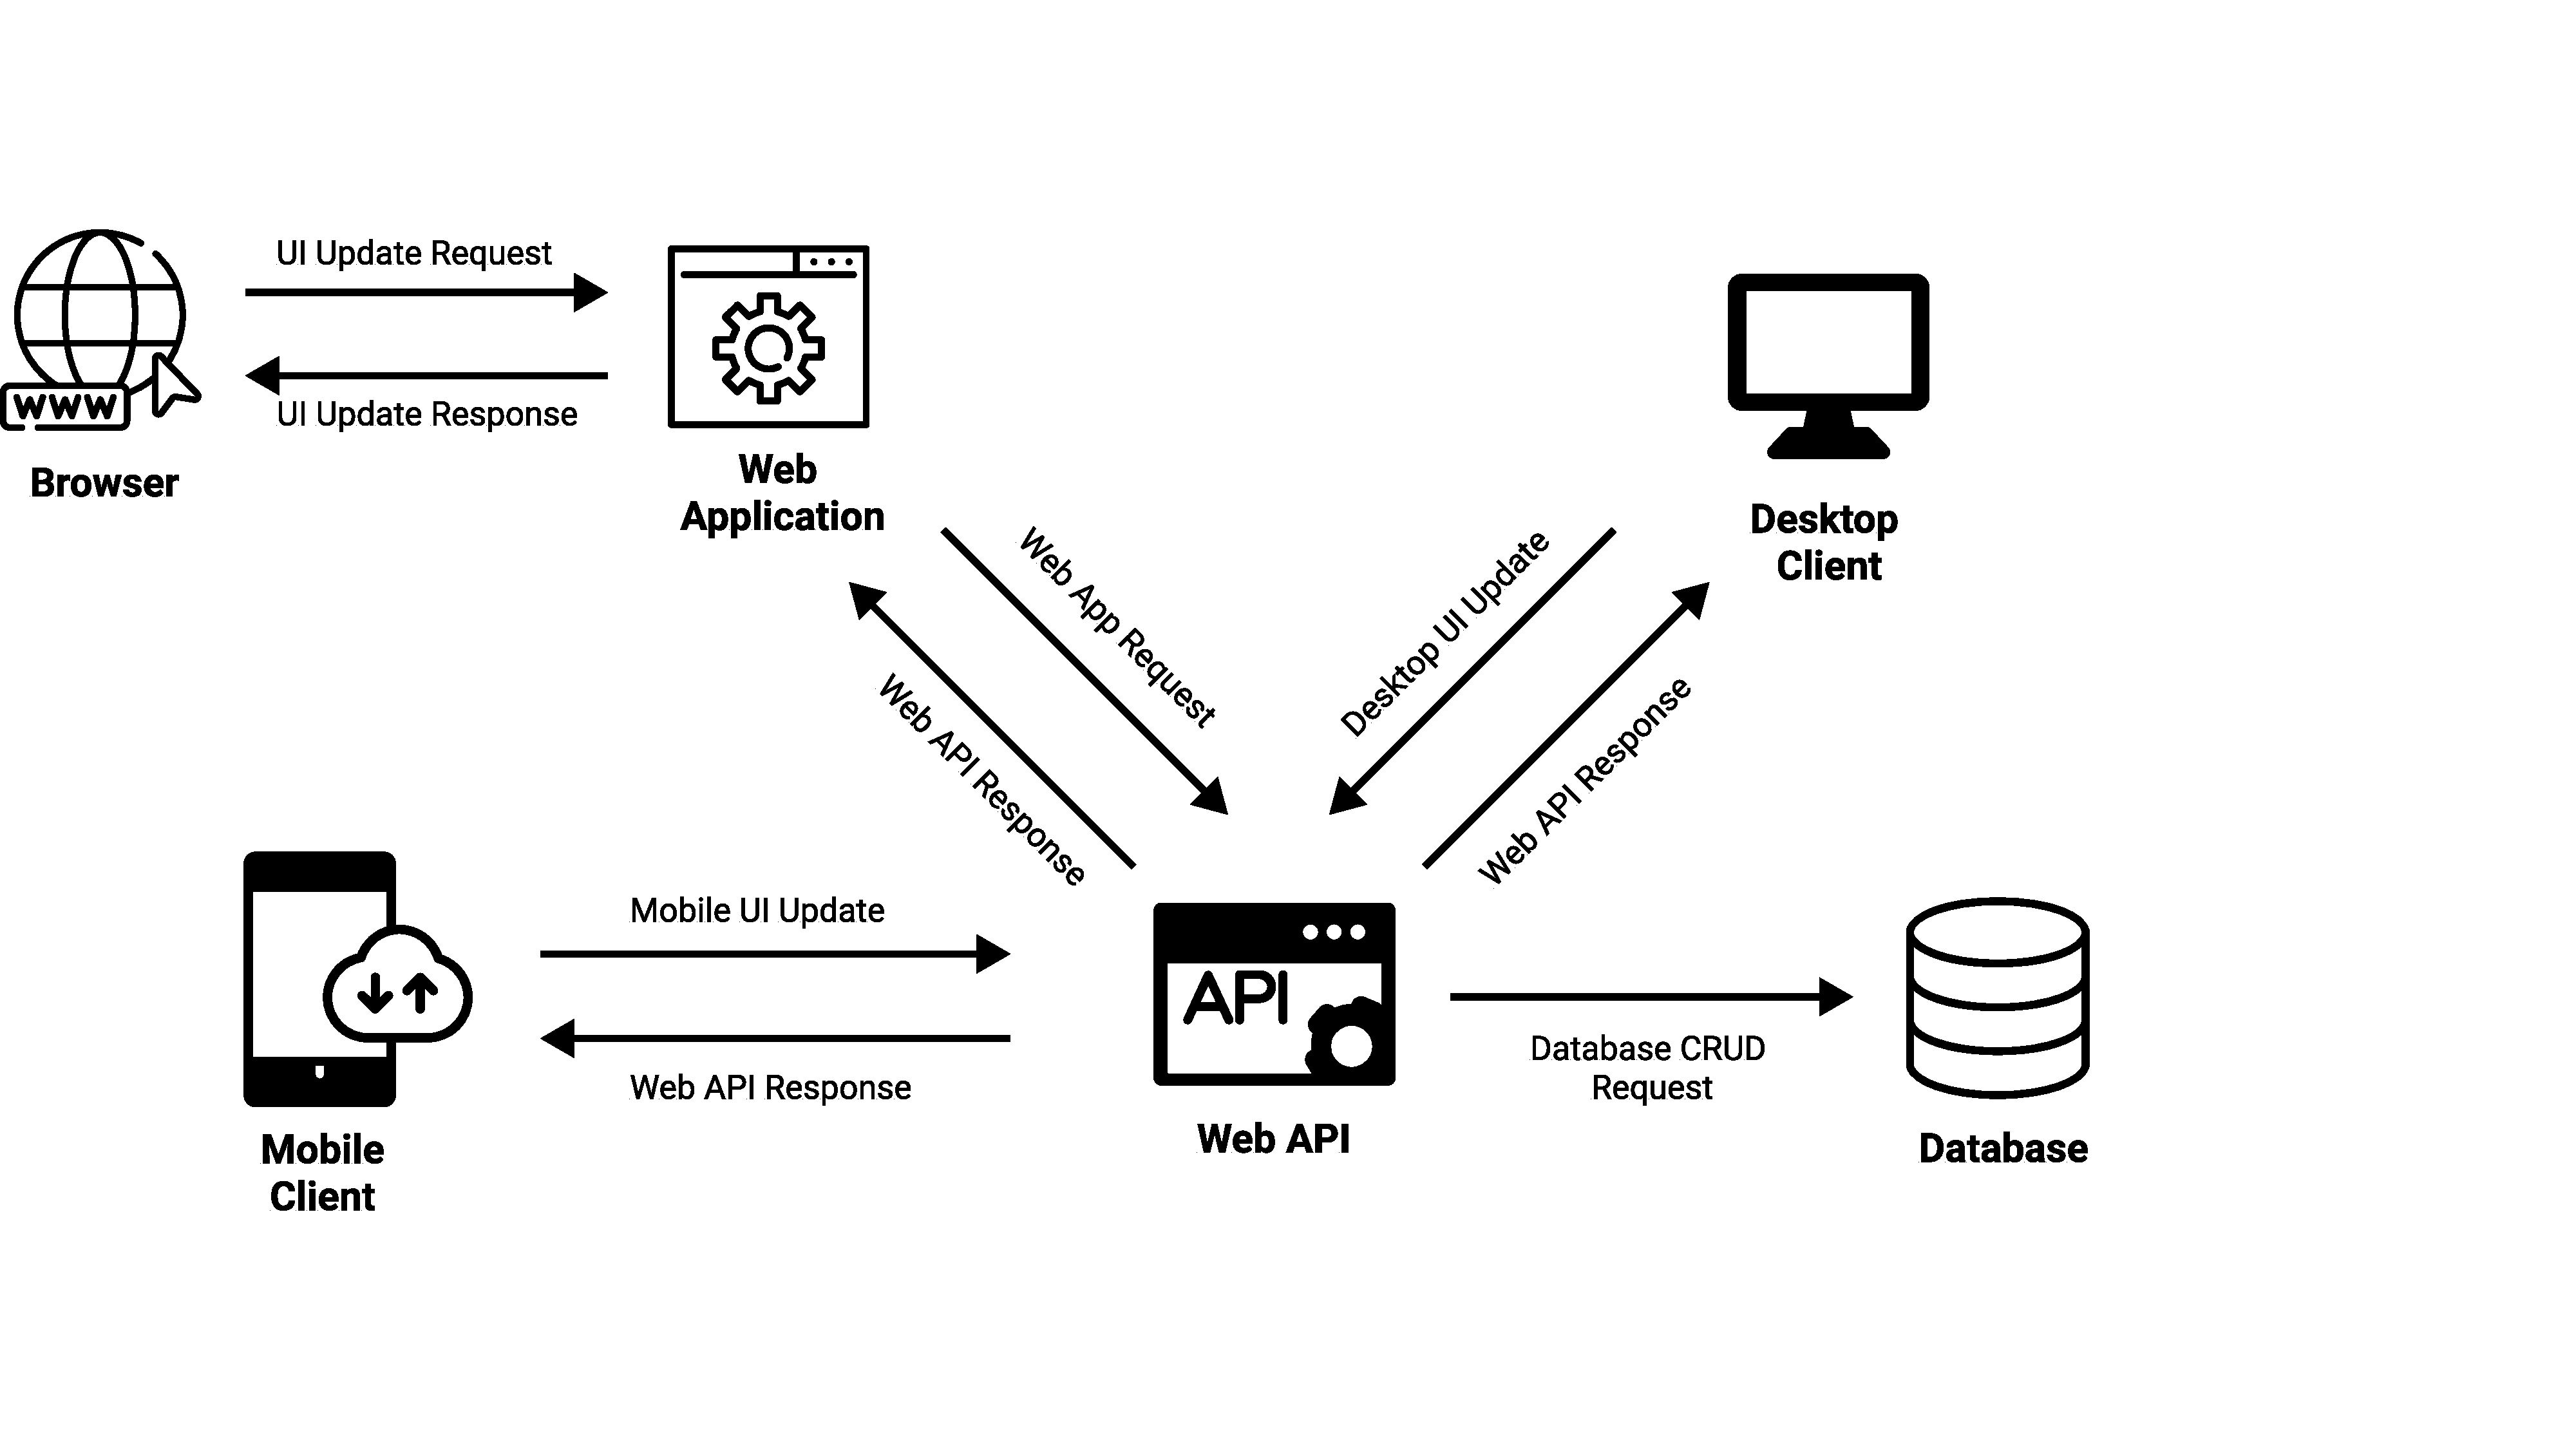
\includegraphics[width=1\textwidth]{Pictures/Threat_Modeling}
    \caption{Database diagram.}\label{fig:figure6}
\end{figure}

Hence, communication between software components is structured as follows

Web Browser - Web Application - Server - Database

- The web browser will send a request to update the interface to the web application
- The web application broadcasts the request to the server
- The server executes business logic and checks access rights, referring to the database
- The server responds to the web application
- Browser user interface updated

Desktop Client - Server - Database

- Desktop client sends a request to update the user interface
- The server executes business logic and checks access rights, referring to the database
- Server responds to desktop client
- Desktop app UI updated as per response from server

Mobile Client - Server - Database

- The mobile client sends a request to update the user interface
- The server executes business logic and checks access rights, referring to the database
- Server responds to desktop client
- The user interface of the mobile app has been updated according to the response from the server

However, such a communication model can carry certain security vulnerabilities, which are discussed below.
Consider communication Web browser - Web application - Server - Database, the first vulnerability that comes to mind
this is phishing.
An attacker could launch his own web application consuming the same web server, thus
it is possible to log user actions and get personal data or an account.
This vulnerability is addressed using a properly configured Cross-Origin Resource Sharing policy that will restrict
Possibility of queries from domains that do not meet the policy.
Like, for instance, it is done in our project

\begin{spverbatim}
    public static void Configure(
    IApplicationBuilder app,
    IWebHostEnvironment env)
    {
        ...

        app.UseCors(CorsPolicy);

        ...
    }

    public void ConfigureServices(IServiceCollection services)
    {
        ...

        services.AddCors(options =>
        {
            options.AddPolicy(CorsPolicy, builder =>
            {
                var allowedOrigins = Configuration
                        .GetSection("AllowedOrigins")
                        .Get<string[]>();

                builder.WithOrigins(allowedOrigins)
                       .AllowAnyMethod()
                       .AllowCredentials()
                       .AllowAnyHeader();
            });
        });

        ...
    }
\end{spverbatim}

The next potential vulnerability is a misconfigured TLS / SSL certificate or a self-signed certificate,
to eliminate the vulnerability of the TLS certificate, you must follow the instructions and
\href{https://www.ssl.com/guide/ssl-best-practices/}{best practices}.
In addition, a potential vulnerability lies in the possibility of SQL injection;
this vulnerability is eliminated by using
parameters in string literals of the SQL query to the database, you should also pay attention to the configuration used
ORM\@.
There is also the danger of an attacker receiving information about the application device through the error logs in the
response from the server, thus, it is recommended to use the unified \href{https://datatracker.ietf.org/doc/html/rfc7231}{response format}
from the server, which, in case of an error, will not contain the details of the error.
It is also recommended using the system of roles for users in order to restrict an unauthorized client from using
resources available only to administrators.

%\begin{enumerate}
%    \item \textbf{Browser UI Update Request}
%    \begin{itemize}
%        \item \textbf{Treat 1.1.} An adversary can perform action on behalf of other user due to lack of controls
%        against cross domain requests.
%        \item \textbf{Treat 1.5.} An adversary can spoof the target web application due to insecure TLS certificate configuration.
%        \item \textbf{Treat 1.8.} An adversary can gain access to sensitive data by performing SQL injection through Web App.
%        \item \textbf{Treat 1.10.} An adversary can deface the target web application by injecting malicious code or uploading dangerous files.
%        \item \textbf{Treat 1.11.} An adversary may spoof Desktop Web Browser (Chrome) and gain access to Web Application.
%        \item \textbf{Treat 1.12.} An adversary can create a fake website and launch phishing attacks.
%        \item \textbf{Treat 1.18.} An adversary can gain access to sensitive information through error messages.
%        \item \textbf{Treat 1.19.} An adversary can gain access to sensitive data by sniffing traffic to Web Application.
%    \end{itemize}
%    \item \textbf{Web App Request}
%    \begin{itemize}
%        \item \textbf{Treat 2.1.} An adversary may gain unauthorized access to Web API due to poor access control checks.
%        \item \textbf{Treat 2.2.} An adversary can gain access to sensitive information from an API through error messages.
%        \item \textbf{Treat 2.3.} An adversary can gain access to sensitive data by sniffing traffic to Web API\@.
%        \item \textbf{Treat 2.5.} Attacker can deny a malicious act on an API leading to repudiation issues.
%        \item \textbf{Treat 2.6.} An adversary may spoof Mango Web Application and gain access to Web API\@.
%        \item \textbf{Treat 2.7.} An adversary may inject malicious inputs into an API and affect downstream processes.
%        \item \textbf{Treat 2.8.} An adversary can gain access to sensitive data by performing SQL injection through Web API\@.
%    \end{itemize}
%    \item \textbf{Web API Response}
%    \begin{itemize}
%        \item \textbf{Treat 3.3.} An adversary can gain access to sensitive information through error messages.
%        \item \textbf{Treat 3.5.} An adversary can spoof the target web application due to insecure TLS certificate configuration.
%        \item \textbf{Treat 3.6.} An adversary can steal sensitive data like user credentials.
%        \item \textbf{Treat 3.7.} An adversary can create a fake website and launch phishing attacks.
%    \end{itemize}
%    \item \textbf{CRUD Request}
%    \begin{itemize}
%        \item \textbf{Treat 4.1.} An adversary can gain unauthorized access to database due to loose authorization rules.
%        \item \textbf{Treat 4.2.} An adversary can gain access to sensitive PII or HBI data in database.
%        \item \textbf{Treat 4.3.} An adversary can gain access to sensitive data by performing SQL injection.
%        \item \textbf{Treat 4.4.} An adversary can deny actions on database due to lack of auditing.
%        \item \textbf{Treat 4.5.} An adversary can tamper critical database securables and deny the action.
%        \item \textbf{Treat 4.7.} An adversary can gain unauthorized access to database due to lack of network access protection.
%    \end{itemize}
%    \item \textbf{Mobile UI Update}
%    \begin{itemize}
%        \item \textbf{Treat 5.1.} An adversary can gain access to sensitive data by performing SQL injection through Web API.
%        \item \textbf{Treat 5.2.} An adversary can reverse engineer and tamper binaries.
%        \item \textbf{Treat 5.3.} An adversary may inject malicious inputs into an API and affect downstream processes.
%        \item \textbf{Treat 5.4.} An adversary may spoof Mobile App (IOS, Android) and gain access to Web API\@.
%        \item \textbf{Treat 5.5.} An adversary obtains refresh or access tokens from Mobile App (IOS, Android) and uses them to
%        obtain access to the Mango Web API\@.
%        \item \textbf{Treat 5.6.} Attacker can deny a malicious act on an API leading to repudiation issues.
%        \item \textbf{Treat 5.7.} An adversary can gain access to sensitive data stored in Web API's config files.
%        \item \textbf{Treat 5.8.} An adversary can gain sensitive data from mobile device.
%        \item \textbf{Treat 5.9.} An adversary can gain access to sensitive data by sniffing traffic to Web API\@.
%        \item \textbf{Treat 5.10.} An adversary can gain access to sensitive data by sniffing traffic from Mobile client.
%        \item \textbf{Treat 5.11.} An adversary can gain access to sensitive information from an API through error messages.
%        \item \textbf{Treat 5.12.} An adversary may gain unauthorized access to Web API due to poor access control checks.
%        \item \textbf{Treat 5.13.} An adversary may jail break into a mobile device and gain elevated privilege.
%    \end{itemize}
%\end{enumerate}